


\documentclass[11pt]{article}
\usepackage[margin=1in]{geometry}
\usepackage{fancyhdr}
\usepackage{amsmath , amsthm , amssymb}
\usepackage{graphicx}
\usepackage{hyperref}
\usepackage{authblk}
\usepackage{setspace}
\usepackage[dvipsnames]{xcolor}

\usepackage{lscape} %this is to make the landscape of individual table pages.
\usepackage{enumitem, float, booktabs}
\setcounter{MaxMatrixCols}{10}

\pagestyle{fancy}
\lhead{}
\chead{}
\rhead{}
\lfoot{}
\cfoot{\thepage}
\rfoot{}
\setlength{\parindent}{0.5in}
\geometry{left=.8in,right=1in,top=1in,bottom=1in}
\renewcommand{\baselinestretch}{2}
\begin{document}

\begin{onehalfspacing}

\begin{center}
\textbf{EC 320: Introduction to Econometrics} \bigskip

\textbf{Problem Set\bigskip\ 1}
\bigskip
\end{center}


\noindent \textbf{Total:  points}

\noindent \textbf{Due: On canvas, January 17th at 5 pm}

\bigskip

\noindent \textbf{Learning Outcomes:}
\begin{itemize}
\item Understanding random variables and probabilities  
\item Understanding bias and variance of estimators 
\item Basic data summary and visualization
\end{itemize}

\bigskip


\noindent \textbf{Checklist Before Handing In:}
\begin{itemize}
\item Did you answer all questions?
\item Did you answer all parts for each question?
\item Were your answers too vague? If so, make them more precise to make sure they really answer the question being asked.
\end{itemize}

\bigskip

\noindent {\textbf{Instructions:}}\ You are encouraged to work with other students in the class, but you must provide original responses. To receive full credit, justify your answers and list your collaborators. For full credit on the computational exercises, include your code and output in addition to your answers. You will turn in digital copies of your responses on Canvas. Please note the list of acceptable file types on the submission page. Finally, you can earn up to 5 extra credit points by typing your responses, or having a clear, neat, well-formatted assignment. \\
\vspace{0.1in}

Name: 			\\
\vspace{0.1in}

Collaborator 1: \\

\vspace{0.1in}

Collaborator 2: 
			
			

\newpage


\begin{center}
\textbf{Analytical Questions} \bigskip
\end{center}


\begin{enumerate}
	
\item Consider an experiment where you flip three fair coins, record whether each coin landed heads or tails, and assign heads a value of 2 and tails a value of -1. You then multiply the values from each flip and describe this product as the random variable $X$. For example, if the coins landed \texttt{heads}, \texttt{heads}, \texttt{tails}, then you would multiply $2 \cdot 2 \cdot -1$ to find an outcome of $X = -4$.
\begin{enumerate}[label=(\alph*)]
	\item Is $X$ a discrete or continuous random variable?\\
	
	\textcolor{PineGreen} {$X$ is a discrete random variable.}\\
	\item Outline the probability distribution of $X$ in a table.\\
		\begin{table}[htb]
		\centering
		
		\begin{tabular}{@{\extracolsep{1cm}} c c c @{}}
			\toprule
			\textcolor{PineGreen}{\textbf{Outcomes}} & \textcolor{PineGreen}{\textbf{$X$}} & \textcolor{PineGreen}{\textbf{Probability}}  \\ \toprule
			\textcolor{PineGreen}{HHH} & \textcolor{PineGreen}{8} & \textcolor{PineGreen}{1/8} \\
			\textcolor{PineGreen}{HTT, TTH, THT} &\textcolor{PineGreen}{2} & \textcolor{PineGreen}{3/8} \\
			\textcolor{PineGreen}{TTT} &\textcolor{PineGreen}{-1} & \textcolor{PineGreen}{1/8} \\
			\textcolor{PineGreen}{HHT, THH, HTH} & \textcolor{PineGreen}{-4} & \textcolor{PineGreen}{3/8} \\
			\bottomrule
		\end{tabular}
	\end{table}
	\item What is the population mean of $X$? In other words, what is $E(X)$?\\
	
	\textcolor{PineGreen} {$E(X) = 8 \cdot 1/8 + 2 \cdot 3/8 - 1 \cdot 1/8 - 4 \cdot 3/8 = 1/8$}\\
	\item What is the population variance of $X$?\\
	
	\textcolor{PineGreen}{ $\mathop{\text{Var}}(X) = E(X^2) - [E(X)]^2 = 8^2 \cdot 1/8 + 2^2 \cdot 3/8 + (-1)^2 \cdot 1/8 + (-4)^2 \cdot 3/8 - (1/8)^2 = 15.625 - 0.015625 = 15.609375$.}
	
\end{enumerate}

\bigskip

\item Consider the distributions of three estimators of the population mean $\mu$:

\begin{figure}[H]
	\centering
	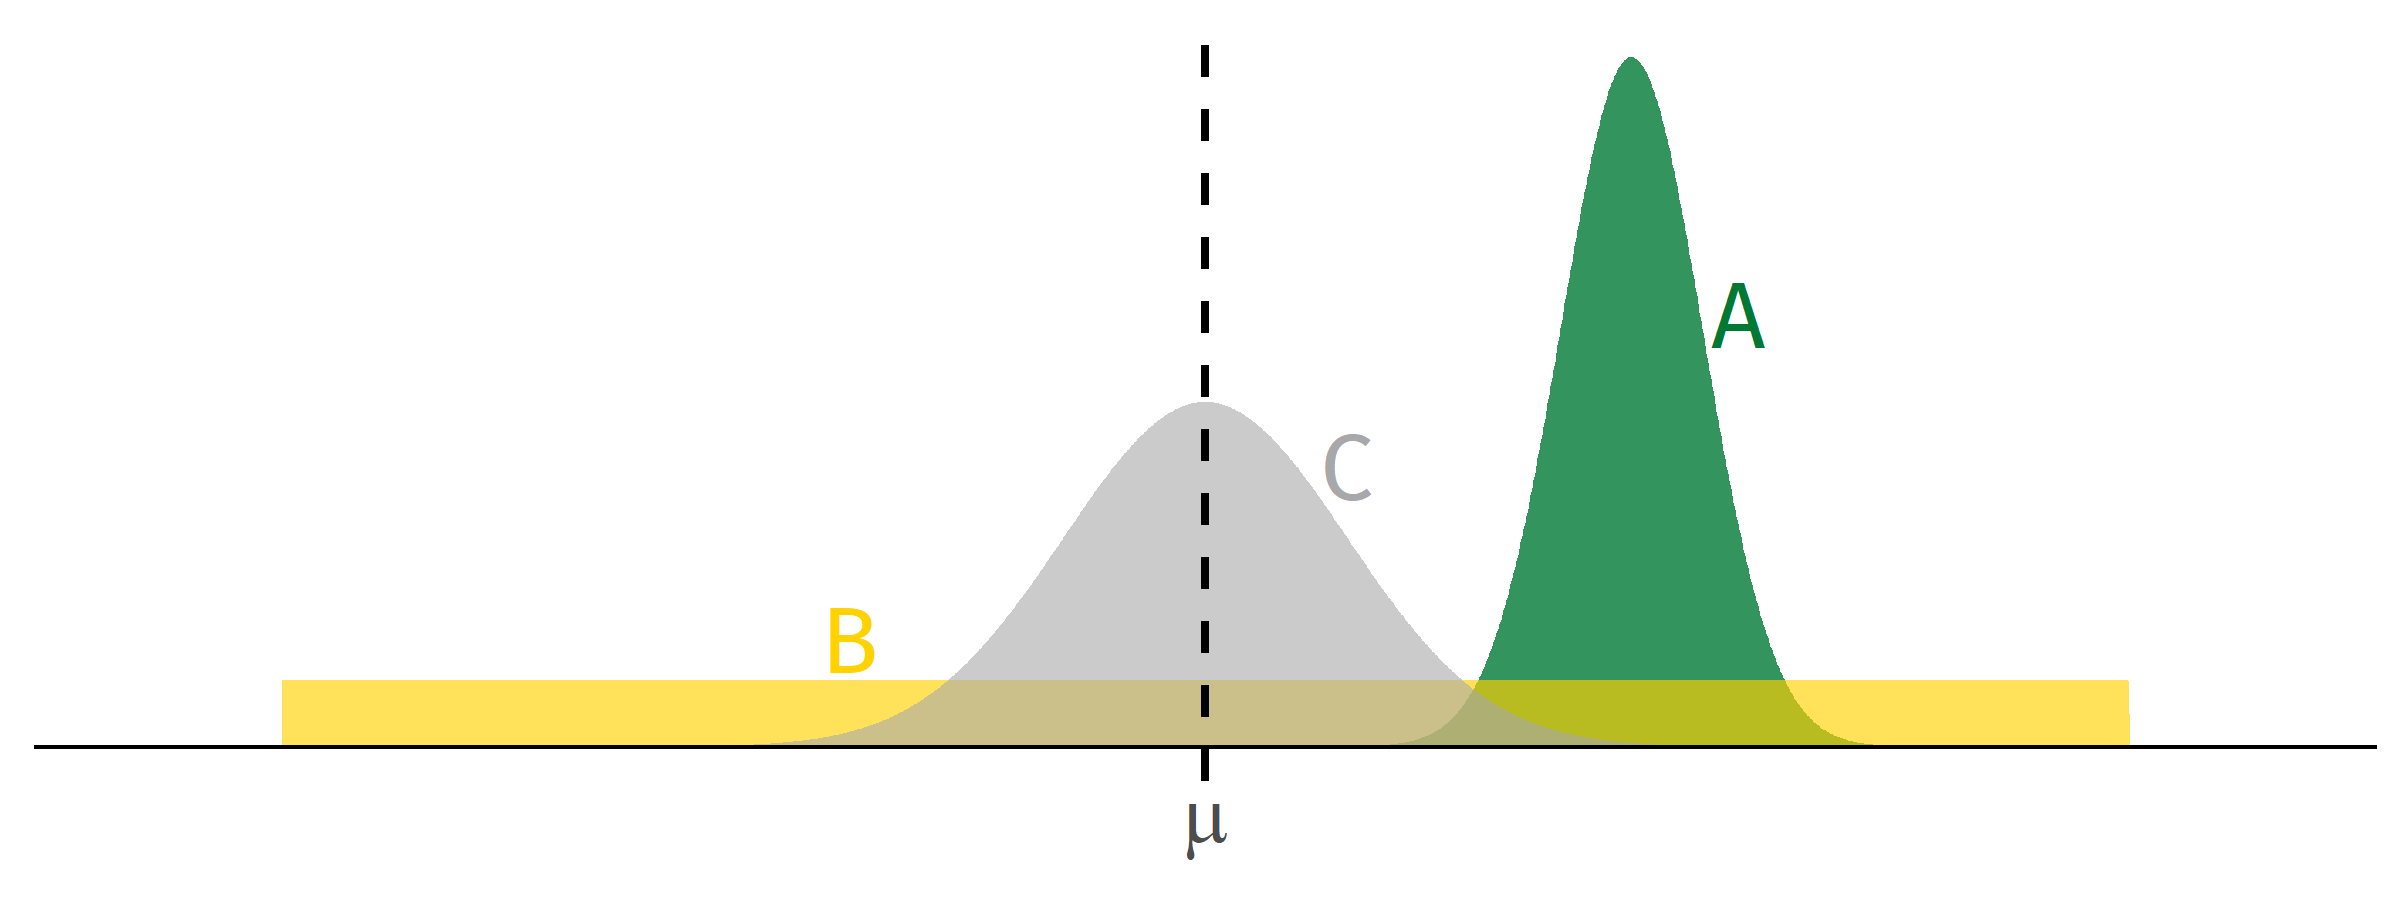
\includegraphics[width=\textwidth]{estimators.png}
	\caption*{\textbf{Note}: Shows the distributions of three estimators (A, B, and C) that provide estimates of the unkown population parameter $\mu$. $E(A) = \mu + 3$,  $E(B) = \mu$, and  $E(C) = \mu$.}
\end{figure}

\begin{enumerate}[label=(\alph*)]
	\item Which of the estimators above is unbiased?\\
	
	\textcolor{PineGreen} {Estimators B and C are unbiased because their expected values are equal to the unknown population parameter $\mu$.}\\
	
	\item  Which of the estimators above has the smallest variance?\\
	
	
	\textcolor{PineGreen}{Of the three estimators, Estimator A has the smallest variance. Compared to those of the other estimators, the estimates from Estimator A are more tightly distributed around the estimator's expected value.}\\
	
	\item Which of the estimators above is the ``best'' unbiased estimator?\\
	
	\textcolor{PineGreen}{The ``best'' unbiased estimator is the unbiased estimator with the least variance. Both Estimator B and Estimator C are unbiased, but Estimator C has a smaller variance. In this sense, Estimator C is the best unbiased estimator.}
\end{enumerate}

\bigskip

\item Use the rules of the expected values operator to \textbf{prove} that the population variance $E \left[ \left( X - E(X) \right)^2 \right]$ is equivalent to $E(X^2) - \left[ E(X)\right]^2$.\\


\textcolor{PineGreen}{
	\begin{align*}
	E[(X-E(X))^2] &= E[(X-E(X)) (X-E(X))]
	\\ &=E[X^2 - 2XE(X) + E(X)^2]
	\\ &= E(X^2) - 2E(X)E(X) + E(X)^2
	\\ &= E(X^2) - E(X)^2
	\end{align*}
}\\

\item Consider data gathered from students on the number of hours they slept the night before their midterm exam and their subsequent exam scores:

\begin{table}[htb]
	\centering
	\begin{tabular}{@{\extracolsep{1cm}} c c c @{}}
		\toprule
		\textbf{Student} & \textbf{Hours Slept} & \textbf{Exam Score}  \\ \toprule
		Ahmed & 8 & 95\% \\
		Chen & 10 & 85\% \\
		Klara & 7 & 70\% \\
		Peter & 4 & 60\% \\
		\bottomrule
	\end{tabular}
\end{table}

\begin{enumerate}[label=(\alph*)]
	\item In the space provided below, draw a scatter plot with \textbf{Exam Score} on the $Y$-axis and \textbf{Hours Slept} on the $X$-axis. Do they appear positively or negatively correlated?\\
	
	\begin{figure}[H]
		\centering
		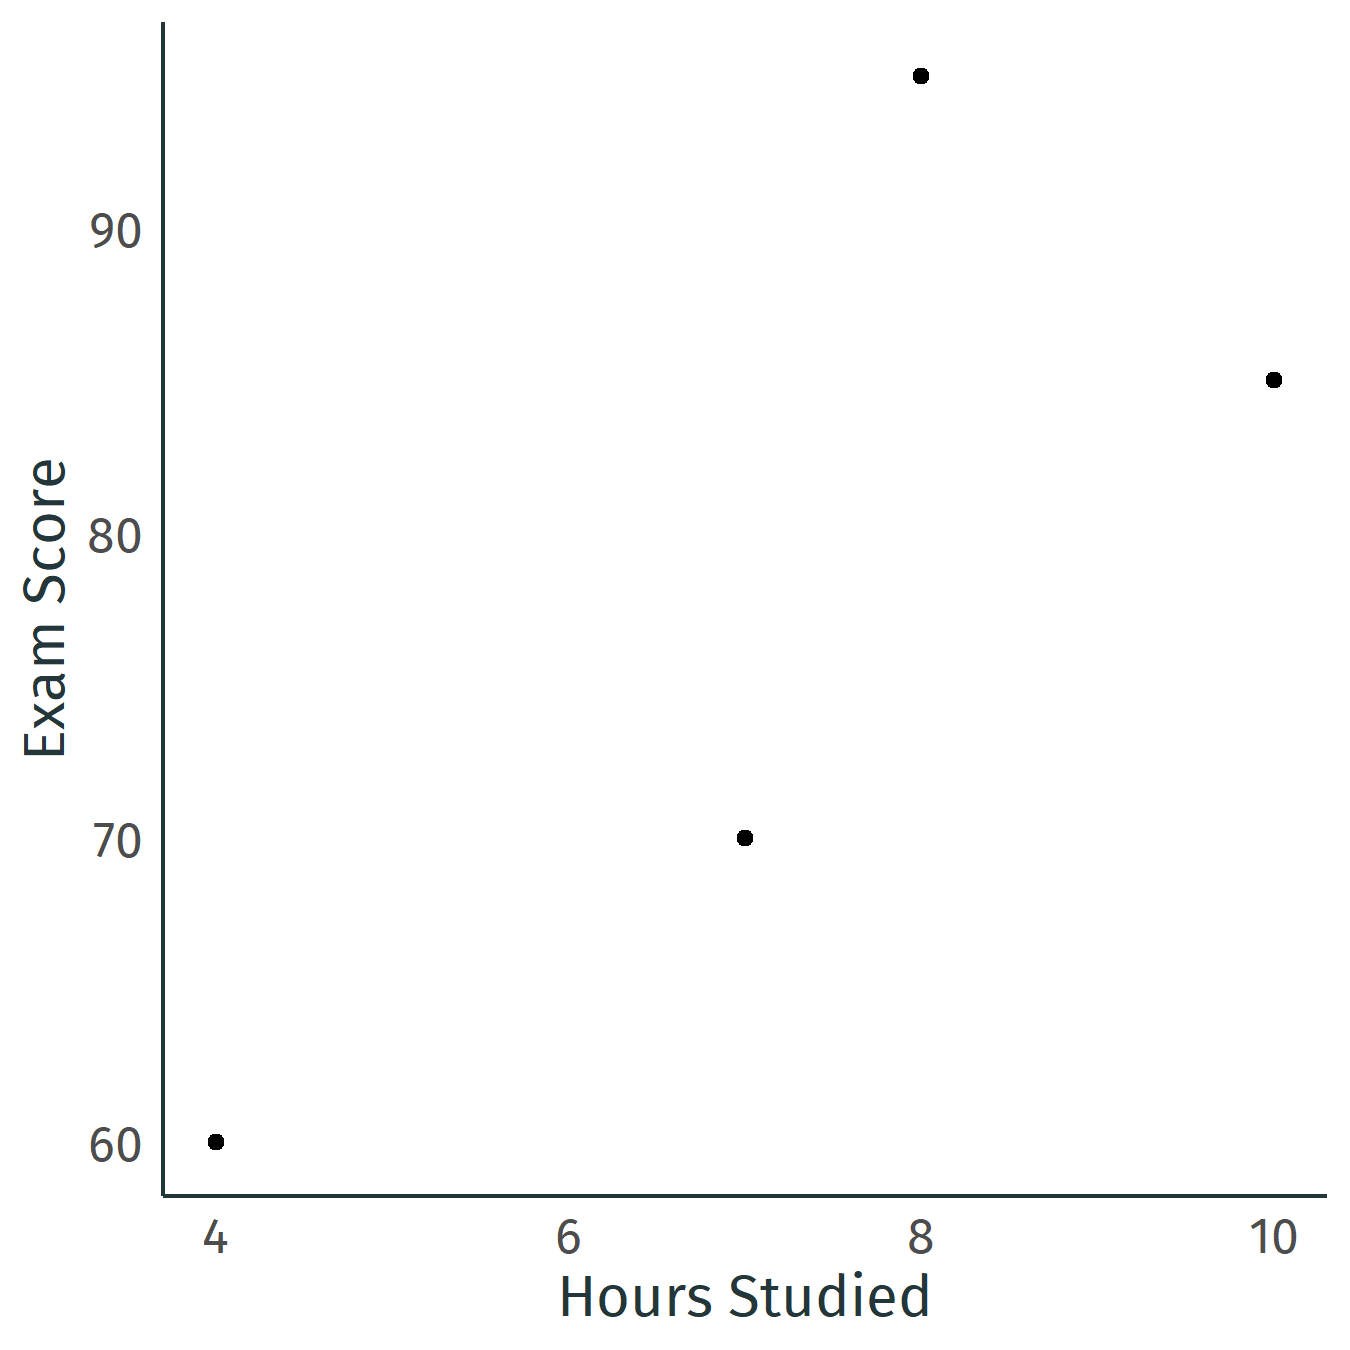
\includegraphics{scatter1.png}
	\end{figure}

	\textcolor{PineGreen} {They appear positively correlated.}\\
	
	\item What is the sample mean of \textbf{Exam Score}?\\
	
	\textcolor{PineGreen}{The mean \textbf{exam score} is 77.5.
	\begin{align*}
	\overline{\text{Exam Score}} &= \frac{95 + 85 + 70 + 60}{4}
	\\ &= \frac{310}{4}
	\\ &= 77.5
	\end{align*}} \\
	
	\item What is the sample variance of \textbf{Hours Slept}?\\
	
	\textcolor{PineGreen}{ The variance of \textbf{hours slept} is 6.25.	
	To calculate the variance, you first need to calculate the sample mean of \textbf{hours slept}:	
	\begin{align*}
	\overline{\text{Hours Slept}} &= \frac{8+10+7+4}{4}
	\\ &= \frac{29}{4}
	\\ &= 7.25.
	\end{align*}
	Then you calculate the sample variance:
	\begin{align*}
	\mathop{\text{Var}}(\text{Hours Slept}) &= \frac{(8 - 7.25)^2 + (10 - 7.25)^2 + (7 - 7.25)^2 + (4 - 7.25)^2 }{4-1}
	\\ &= \frac{0.5625 + 7.5625 + 0.0625 + 10.5625}{4-1}
	\\ &= \frac{18.75}{3}
	\\ &= 6.25.
	\end{align*}	}
	
	\item What is the sample correlation coefficient between \textbf{Exam Score} and \textbf{Hours Slept}?\\
	
\textcolor{PineGreen}{ The correlation between \textbf{exam score} and \textbf{hours slept} is approximately 0.79.
	Start by calculating the sample covariance between \textbf{exam score} and \textbf{hours slept}:
	\scriptsize
	\begin{align*}
	\mathop{\text{Cov}}(\text{Score}, \text{Sleep}) &= \frac{(8 - 7.25)(95 - 77.5) + (10 - 7.25)(85 - 77.5) + (7 - 7.25)(70 - 77.5) + (4 - 7.25)(60 - 77.5) }{4-1}
	\\ &= \frac{13.125 + 20.625 + 1.875 + 56.875}{4-1}
	\\ &= \frac{92.5}{3}
	\\ &\approx 30.83.
	\end{align*}	
	\normalsize	
	The correlation coefficient is given by
	\begin{align*}
	\mathop{\text{Cor}}(\text{Exam Score}, \text{Hours Slept}) &= \frac{\mathop{\text{Cov}}(\text{Exam Score}, \text{Hours Slept})}{\sqrt{\mathop{\text{SD}}(\text{Exam Score})} \cdot \sqrt{\mathop{\text{SD}}(\text{Hours Slept})}}.
	\end{align*}
	To find the standard deviations, you need the variances. 
	Calculate the sample variance of \textbf{Exam Score}:	
	\begin{align*}
	\mathop{\text{Var}}(\text{Exam Score}) &= \frac{(95 - 77.5)^2 + (85 - 77.5) ^2 + (70 - 77.5)^2 + (60 - 77.5)^2 }{4-1}
	\\ &= \frac{725}{4-1}
	\\ &= \frac{725}{3}
	\\ &\approx 241.67.
	\end{align*}	
	Finally, you can plug in what you know:	
	\begin{align*}
	\mathop{\text{Cor}}(\text{Exam Score}, \text{Hours Slept}) &= \frac{\mathop{\text{Cov}}(\text{Exam Score}, \text{Hours Slept})}{\sqrt{\mathop{\text{SD}}(\text{Exam Score})} \cdot \sqrt{\mathop{\text{SD}}(\text{Hours Slept})}}
	\\ &= \frac{30.83}{\sqrt{6.25} \cdot \sqrt{241.67}}
	\\ &= \frac{30.83}{2.5 \cdot 15.54574}
	\\ &\approx 0.79.
	\end{align*}	
	}
\end{enumerate}

\end{enumerate}

\newpage 

\begin{center}
\label{Computational}
\textbf{Computational Questions} \bigskip
\end{center}

\noindent For this portion of the problem set, you will use the file \texttt{election\_2016.csv} in the \texttt{Problem\_Set\_1} folder on Canvas. The file contains county-level data on the 2016 presidential election from the \href{https://electionlab.mit.edu/data}{MIT Election Data and Science Lab} and the \href{https://www.census.gov/data.html}{US Census Bureau}. You will first need to download the data from Canvas and import it into \texttt{R}. Then you will need to load the \href{https://www.tidyverse.org}{\texttt{tidyverse}} package.

\begin{table}[htb]
	\centering
	\begin{tabular}{@{\extracolsep{1cm}} l l @{}}
		\toprule
		\textbf{Variable Name} & \textbf{Description}  \\ \toprule
		\texttt{stname} & Name of state \\
		\texttt{fips} & County identifier (FIPS code) \\
		\texttt{trump} & Number of votes cast for Donald Trump \\
		\texttt{clinton} & Number of votes cast for Hillary Clinton \\
		\texttt{totalvotes} & Total number of votes cast for any presidential candidate \\
		\texttt{white} & Percentage of eligible voters who are non-Hispanic white \\
		\texttt{poverty} & Percentage of residents below the poverty line  \\
		\texttt{population} & Number of residents \\
		\bottomrule
	\end{tabular}
\end{table}

\noindent Use the data to complete the tasks and questions below.

\begin{enumerate}
	
\item Reduce your data set to include only those counties with a population of 50,000 or more.
	
\item Generate new variables that give the percentage of votes cast for each candidate using the \href{https://dplyr.tidyverse.org/reference/mutate.html}{\texttt{mutate}} function. With these new variables, generate a third variable called \texttt{trump\_margin} that gives Trump's ``margin of victory'' in each county. (For counties that Clinton won, the value of \textbf{\texttt{trump\_margin}} will be negative.)

\item Produce summary statistics (min, max, mean, median, standard deviation, and the number of observations) for \textbf{\texttt{trump\_margin}}, \textbf{\texttt{white}}, \textbf{\texttt{poverty}}, and \textbf{\texttt{population}} using the \href{https://dplyr.tidyverse.org/reference/summarise.html}{\texttt{summarize}} function. Use your summary statistics to answer the following:
\begin{enumerate}[label=(\alph*)]
	\item What is Trump's average vote margin?
	\item What is the median poverty rate?
	\item How many people live in the least populous county? How many live in the most populous county?
\end{enumerate}

\item Create a histogram of Trump's margin of victory. Which candidate won more counties? Is it necessarily the case that this candidate won more votes nationally? \textit{Hint}: Look at a histogram of county population, too.

\item Create a scatter plot with \textbf{\texttt{trump\_margin}} on the $Y$-axis and \textbf{\texttt{poverty}} on the $X$-axis. Does support for Trump appear positively or negatively correlated with poverty rates? Use the \href{https://www.rdocumentation.org/packages/stats/versions/3.6.1/topics/cor}{\texttt{cor}} function to calculate the correlation coefficient. Interpret your result.

\item Create a scatter plot with \textbf{\texttt{trump\_margin}} on the $Y$-axis and \textbf{\texttt{white}} on the $X$-axis. Does support for Trump appear positively or negatively correlated with the percentage of white voters? Use the \texttt{cor} function to calculate the correlation coefficient. Interpret your result.

\item Using \href{https://dplyr.tidyverse.org/reference/group_by.html}{\texttt{group\_by}} and \texttt{summarize}, aggregate the county-level data on \textbf{\texttt{white}}, \textbf{\texttt{poverty}}, and \textbf{\texttt{population}} to the state level. The first two variables are rates. To obtain accurate state-level rates, you need to account for differences in population across counties. You can do this by using the \href{https://www.rdocumentation.org/packages/stats/versions/3.6.1/topics/weighted.mean}{\texttt{weighted.mean}} function inside \texttt{summarize}. For population, you can use the \texttt{sum} function. Your new \href{https://tibble.tidyverse.org}{\texttt{tibble}} should have 50 rows.

\item Using the state-level data, create a scatter plot with \textbf{\texttt{poverty}} on the $Y$-axis and \textbf{\texttt{white}} on the $X$-axis. To illustrate differences in population across states, vary the size of each point by population. You can this by including \texttt{size = population} in the \href{https://ggplot2.tidyverse.org/reference/aes.html}{\texttt{aes}} function of \href{https://ggplot2.tidyverse.org/reference/ggplot.html}{\texttt{ggplot}}. Describe any patterns you see.


\end{enumerate}
\end{onehalfspacing}
\end{document}
